\subsection{Evidence in System State Nodes}
\label{sec:design:bayesian-network:system-state-nodes-evidence}

In \cref{fig:design:bayesian-network:overview} we suggested two nodes that supply information about the system state. The TV\_IsOn supplies information about whether not the television is on and the MusicCentre\_IsPlaying node supplies information on whether or not the music centre is playing music. Naturally these are examples of nodes that can describe the state of the system. Other examples can include if a lamp is on or not, a door is locked or unlocked or who is home.

In \cref{fig:design:bayesian-network:overview} the TV\_IsOn and MusicCentre\_IsPlaying nodes are parents of the System\_State\_Action node. An alternative model for the system state is illustrated in \cref{fig:design:bayesian-network:system-state-nodes-evidence:alternative-network}. 

\begin{figure}[h!]
\centering
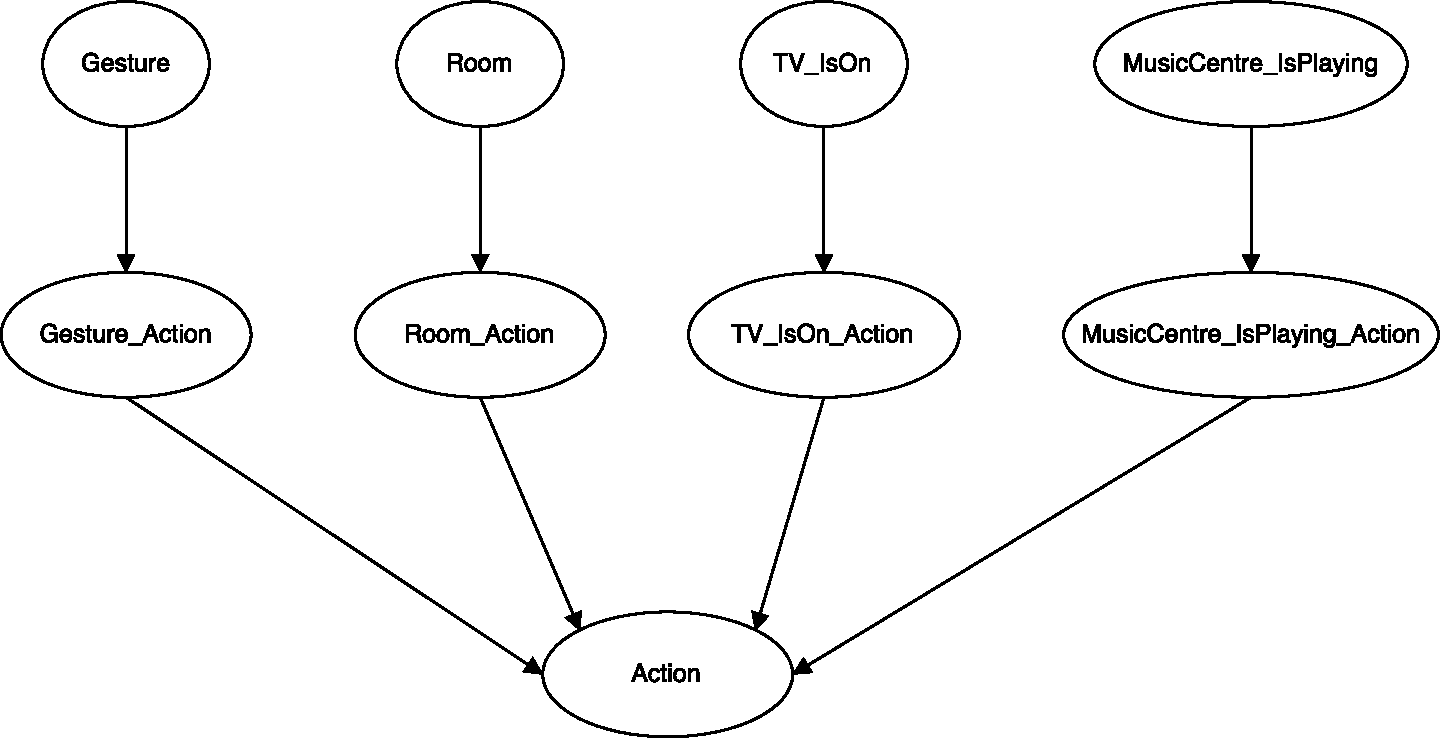
\includegraphics[width=0.75\textwidth]{images/bayesian-network-split-system-state}
\caption{Alternative apporach for modeling the system state in the Bayesian network.}
\label{fig:design:bayesian-network:system-state-nodes-evidence:alternative-network}
\end{figure}

The System\_State action node have been replaced by the TV\_IsOn\_Action and MusicCentre\_IsPlaying\_Action nodes. Each observes a specific part of the system state. The conditional probability tables for the nodes are shown in \cref{tbl:design:bayesian-network:system-state-nodes-evidence:alternative-system-state}.

Consider the table for TV\_IsOn\_Action with a subset of the actions presented in the scenario. As the node knows nothing about the state of the television, it must have equal probabilities for the two states when the television is on. However, if the television is off the node has zero probability of changing the channel on the television. The same principle applies for the MusicCentre\_IsPlaying\_Action node.

\begin{table}[h!]
\centering
\caption{Probability tables for the TV\_IsOn\_Action and MusicCentre\_IsPlaying\_Action nodes in the alternative Bayesian network illustrated in \cref{fig:design:bayesian-network:system-state-nodes-evidence:alternative-network}.}
\label{tbl:design:bayesian-network:system-state-nodes-evidence:alternative-system-state}
\begin{tabular}{cc}
\begin{tabular}{c}
\textbf{TV\_IsOn\_Action}   \\
\begin{tabular}{l|cc}
~ & Yes   & No \\ \hline
Music centre: next track & 0.5 & 1 \\
Television: next channel & 0.5 & 0
\end{tabular}
\end{tabular}
&
\begin{tabular}{c}
\textbf{MusicCentre\_IsPlaying\_Action}   \\
\begin{tabular}{l|cc}
~ & Yes   & No \\ \hline
Music centre: next track & 0.5 & 0 \\
Television: next channel & 0.5 & 1
\end{tabular}
\end{tabular}
\end{tabular}
\end{table}

The influence of the system state is illustrated in \cref{fig:design:bayesian-network:evidence-system-state-nodes:system-state-1,fig:design:bayesian-network:evidence-system-state-nodes:system-state-2}. For readability purposes the illustrated networks only contains a subset of the scenarios presented in \cref{sec:analysis:scenarios}. In the first figure the system state has little influence. The television is on and the music is playing but because the user is in the living room, the action is triggered on the music centre. In the second figure, an action is triggered in the bedroom even though there is evidence that the user is in the living room. The ``Music centre: next track'' is not triggered as the music centre is not playing. However, the gesture has a meaning in the bedroom from which there is little evidence that the user is in. Therefore the action is triggered in the bedroom. Had there been hard evidence that the user is in the living room, the actions would have had the same probability and the system would ask the user which of the two actions he desired to trigger.

\begin{figure}[h!]
\centering
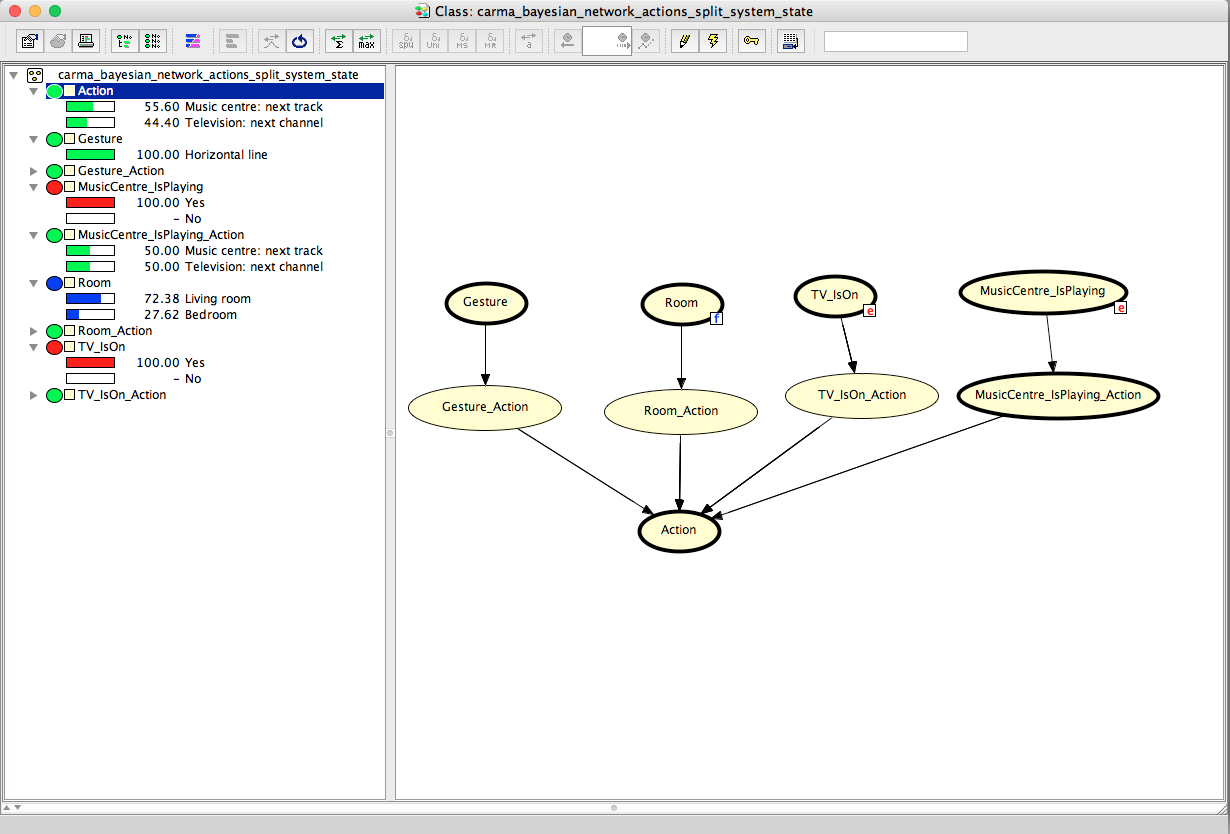
\includegraphics[width=\textwidth]{images/bayesian-split-system-state-1}
\caption{Example Bayesian network with origin in the scenario presented in \cref{sec:analysis:scenarios}. The network has a single gesture, a probability of 72.38\% that the user is in the living room and 27.62\% that he is in the bedroom. The user is in the living room. The television is turned on and the music is playing. Because the user is in the living room, the music is changed when the Horizontal Line gesture is performed. Green bars indicate probabilities, red bars indicate hard evidence and blue bars indicate soft evidence.}
\label{fig:design:bayesian-network:evidence-system-state-nodes:system-state-1}
\end{figure}

\begin{figure}[h!]
\centering
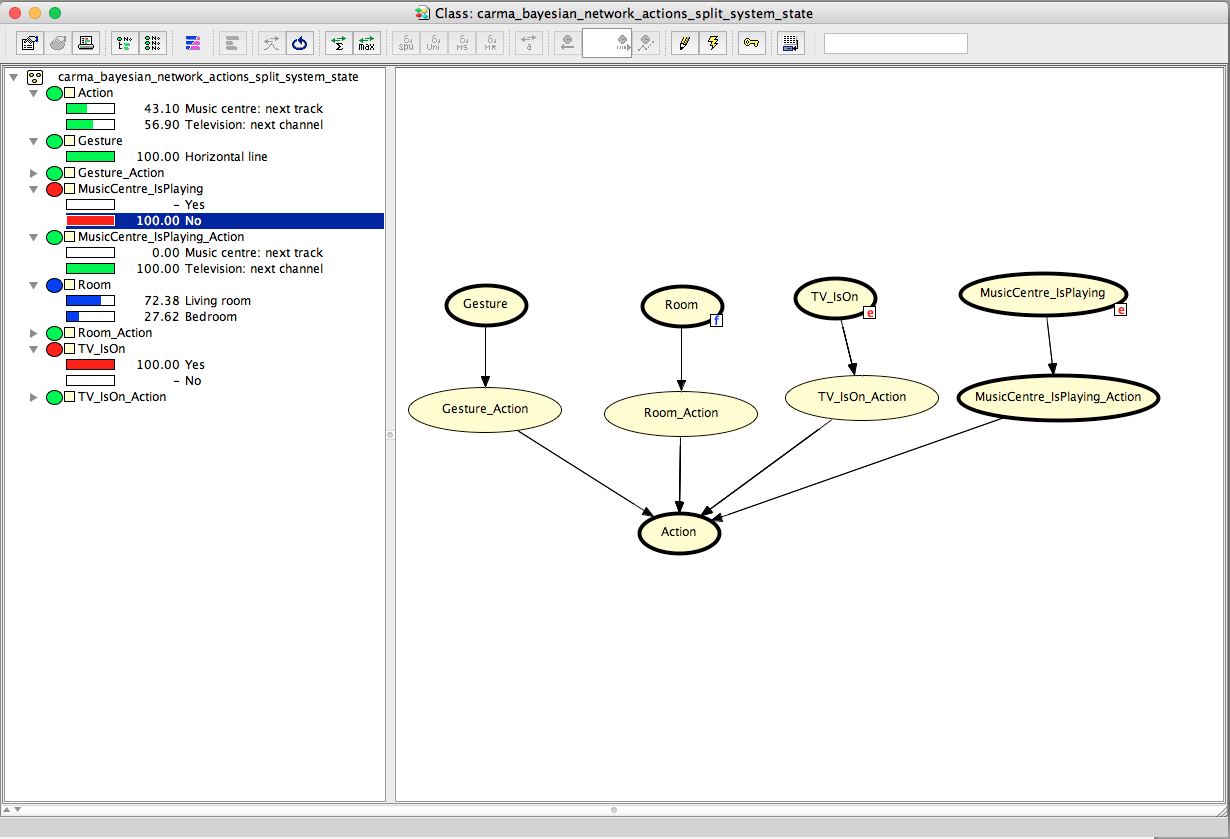
\includegraphics[width=\textwidth]{images/bayesian-split-system-state-2}
\caption{Example Bayesian network with origin in the scenario presented in \cref{sec:analysis:scenarios}. The network has a single gesture, a probability of 72.38\% that the user is in the living room and 27.62\% that he is in the bedroom. While the user is in the living room, the action in the bedroom is performed when the user triggers a gesture because the action in the living room is not valid according to the system state. Green bars indicate probabilities, red bars indicate hard evidence and blue bars indicate soft evidence.}
\label{fig:design:bayesian-network:evidence-system-state-nodes:system-state-2}
\end{figure}

As illustrated in figures \cref{fig:design:bayesian-network:evidence-system-state-nodes:system-state-1,fig:design:bayesian-network:evidence-system-state-nodes:system-state-2} evidence on the system state is hard. The system state can be obtained from the items in openHAB and assuming that we can trust the data delivered by openHAB, we can be sure of the system state.

%%% Local Variables:
%%% mode: latex
%%% TeX-master: "../../master"
%%% End:
